%! suppress = MissingImport
\subsection{Install the \developmentboard onto the Breadboard}

Orient the breadboard in front of you so that row 1 is on your left and row 63 is on your right;
column a should be at the bottom, and column j should be at the top.

Remove the anti-static foam from the \developmentboard's pins.
You will place the \developmentboard\ on the left side of the breadboard with the USB connector on the left (that is, facing away from the breadboard).
Position the upper row of pins on contact points g1-g15 and the lower row of pins on contact points c1-c15.
The left side of the \developmentboard\ will obscure the labels for columns c-g.
The right side of the \developmentboard\ will cover contact points c16-g16 but won't use them.
Double-check that:
\begin{itemize}
    \item the pin labeled \texttt{D12} is in the upper-left, on contact point g1
    \item the pin labeled \texttt{D13} is in the lower-left, on contact point c1
    \item the pin labeled \texttt{VIN} is in the lower-right, on contact point c15
    \item the pin labeled \texttt{TX1} is in the upper-right, on contact point g15
\end{itemize}

Gently press on both ends of the \developmentboard\ to insert the pins into the contact points, using a slight rocking motion if necessary (Figure~\ref{fig:inserting-mcu}).
Press the \developmentboard\ into the breadboard until it physically cannot be inserted any deeper (Figure~\ref{fig:mcu-inserted}).

%! suppress = NonMatchingIf
\begin{figure}
    \centering
    \subfloat[Press gently on both ends of the \developmentboard.] {
        \ifdefstring{\developmentboard}{Arduino Nano}{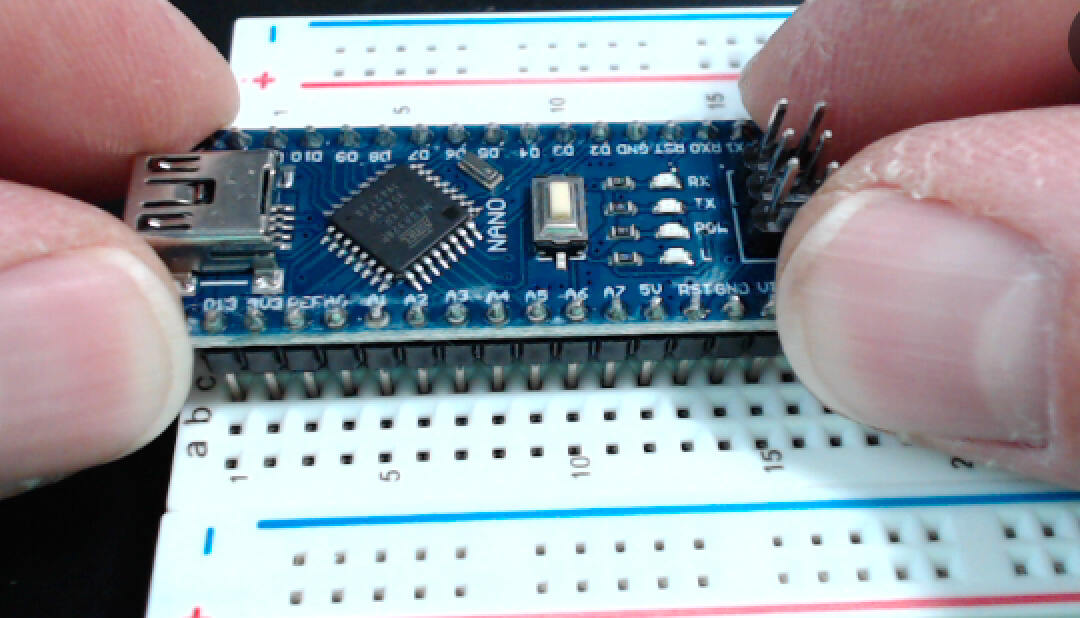
\includegraphics[height=3cm]{microcontroller/breadboard/inserting-nano}}{}
        \label{fig:inserting-mcu}
    }
    \hfil
    \subfloat[The \developmentboard\ fully inserted.] {
        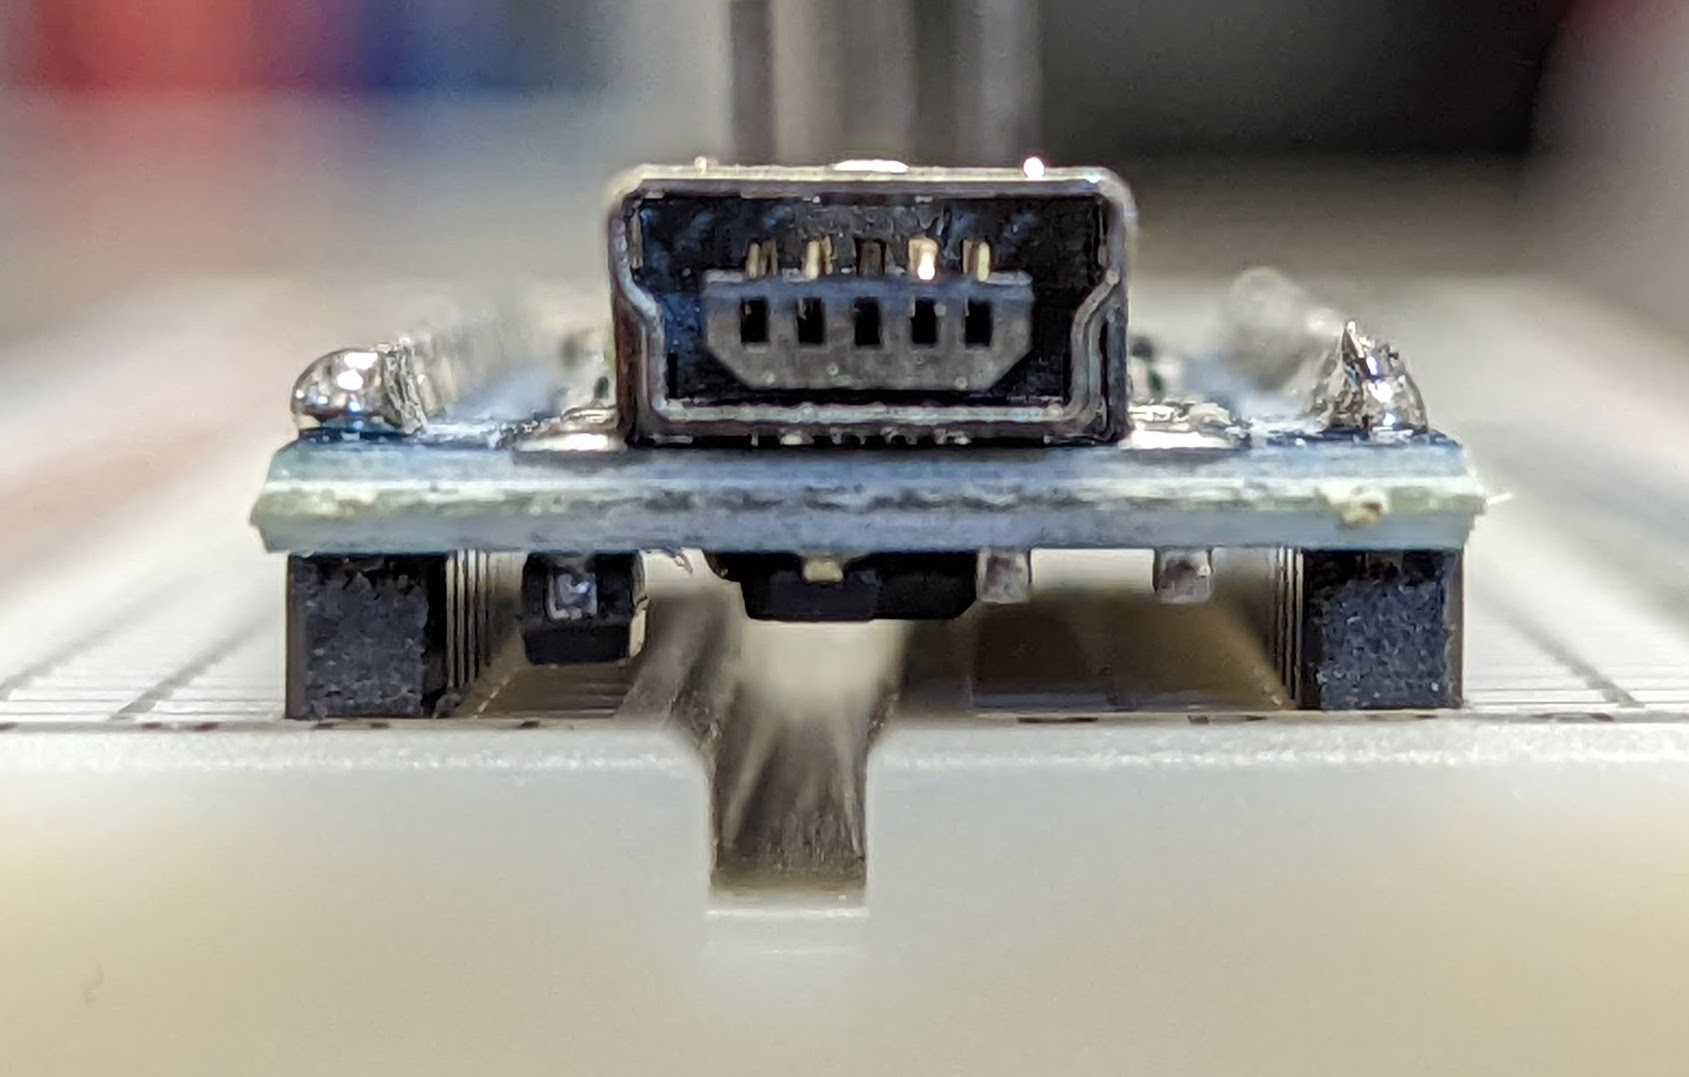
\includegraphics[height=3cm]{microcontroller/breadboard/nano-fully-inserted}
        \label{fig:mcu-inserted}
    }
    \caption{Inserting the \developmentboard\ into the breadboard.}
\end{figure}

\checkpoint{inserted the \developmentboard\ into the breadboard}
